\chapter{ROLLO: Reactor evOLutionary aLgorithm Optimizer}
\label{chap:rollo}
In this chapter, I introduce the \gls{ROLLO} framework. 
\gls{ROLLO} is a Python package that applies evolutionary algorithm 
techniques to optimize nuclear reactor design. 
Applying evolutionary algorithms to nuclear design problems is not new, as I
previously discussed in Section \ref{sec:opt}, and available evolutionary algorithm 
packages can be customized for reactor design optimization problems. 
However, evolutionary algorithm setup is highly customizable with
an assortment of genetic algorithm designs and operators.
A reactor designer unfamiliar with evolutionary algorithms will have
to go through the cumbersome process of customizing a genetic algorithm 
for their needs and determine which operators and hyperparameters work best for 
their problem. 
Furthermore, computing fitness values with nuclear software is computationally 
expensive, necessitating using supercomputers and setting up parallelization 
for the genetic algorithm.

%%% ADD THAT EVOLUTIONARY ALGORITHM OPTIMIZATION TOOL FOR NON CONVENTIONAL DESIGNS 
%%% DOES NOT EXIST. 

Therefore, the motivation behind creating \gls{ROLLO} is to limit these inconveniences and 
facilitate using evolutionary algorithms for reactor design optimization.
\gls{ROLLO} provides a general genetic algorithm framework, sets up 
parallelization for the user, and promotes usability with an input file 
that only exposes mandatory parameters.
\gls{ROLLO} also strives to be effective, flexible, open-source, parallel, reproducible, 
and usable. 
I briefly summarize how \gls{ROLLO} achieves these goals:  
\begin{itemize}
    \item Effective: \gls{ROLLO} is well documented, tested, and 
    version-controlled on Github \cite{chee_rollo_2021}.
    \item Flexible: The proposed work aims to utilize \gls{ROLLO} to 
    explore arbitrary reactor geometries and heterogeneous fuel distributions. 
    However, future users might want to utilize \gls{ROLLO} 
    to explore other arbitrary design parameters. Thus, I designed the \gls{ROLLO}
    framework accordingly. The user can vary any imaginable parameter 
    because \gls{ROLLO} uses a templating method to edit the input file of the 
    coupled software.
    \item Open-source: \gls{ROLLO} utilizes a well-documented, open-source 
    evolutionary algorithm Python package to drive the optimization process, 
    and established open-source nuclear software (OpenMC \cite{romano_openmc_2013} and 
    Moltres \cite{lindsay_introduction_2018}) to compute the objective function 
    and constraints. I also provide a simple tutorial for future developers to 
    follow for coupling other nuclear software to \gls{ROLLO} \cite{chee_documentation_2021}.  
    \item Parallel: Users have the option to run \gls{ROLLO} in parallel using 
    either the \\ \texttt{multiprocessing\_on\_dill} or \texttt{mpi4py} Python 
    packages \cite{dalcin_mpi_2008}.
    \item Reproducible: Data from every \gls{ROLLO} run saves into a unique, pickled 
    file (pickle is a Python module that serializes Python objects), and all 
    results from this work are available on Github. 
\end{itemize}

\gls{ROLLO} essentially couples an evolutionary algorithm driver with nuclear 
software, such as neutron transport and thermal-hydraulics codes. 
Figure \ref{fig:genetic_alg} from Chapter \ref{chap:lit-review} outlines the 
evolutionary algorithm iterative problem solving process. 
I modified Figure \ref{fig:genetic_alg} to produce Figure 
\ref{fig:genetic_alg_nuclear}, which depicts how the nuclear transport and 
thermal-hydraulics software fit within \gls{ROLLO}'s evolutionary algorithm 
optimization process. 
\begin{figure}[]
    \centering
    \begin{tikzpicture}[node distance=1.7cm]
            \tikzstyle{every node}=[font=\small]
            \node (1) [lbblock] {\textbf{Create initial population}};
            \node (2) [loblock, below of=1] {\textbf{Evaluate initial population}};
            \node (3) [lbblock, below of=2, yshift = -1.3cm] {\textbf{Create new population:} \\ 
            \begin{enumerate} \item \textbf{Select} individuals for mating 
                              \item Create offspring by \textbf{crossover} 
                              \item \textbf{Mutate} selected individuals 
                              \item Keep selected individuals from previous generation
                             \end{enumerate}};
            \node (4) [loblock, below of=3, yshift=-1.3cm] {\textbf{Evaluate new population}};
            \node (5) [lbblock, below of=4] {\textbf{Is termination \\ criteria satisfied?}};
            \node (6) [lbblock, below of=5] {\textbf{Best solution is returned!}};
            \draw [arrow] (1) -- (2);
            \draw [arrow] (2) -- (3);
            \draw [arrow] (3) -- (4);
            \draw [arrow] (4) -- (5);
            \draw [arrow] (5) -- node[anchor=east] {yes} (6);
            \draw [arrow] (5) -- ([shift={(0.5cm,0cm)}]5.east)-- node[anchor=west] {no} ([shift={(0.5cm,0cm)}]3.east)--(3);
            \matrix [draw,above right,yshift=10.7cm, xshift=0cm] at (current bounding box.south east) {
            \node [bbblock,label=right:\textbf{EA: Evolutionary Algorithm}] {}; \\
            \node [boblock,label=right:\textbf{NS: Nuclear Software}] {}; \\
            };
    \end{tikzpicture}
    \caption{Process of finding optimal solutions for a problem with a 
    genetic algorithm. Nuclear software evaluates each new population.}
    \label{fig:genetic_alg_nuclear}
\end{figure}
\gls{ROLLO} initially reads and validates the JSON input 
file, initializes the \gls{DEAP} \cite{fortin_deap_2012} genetic algorithm 
hyperparameters and operators, and finally runs the genetic algorithm following 
the flow chart in Figure \ref{fig:genetic_alg_nuclear}, in which the nuclear 
software evaluates each individual's fitness. 

In the subsequent sections, I describe the evolutionary algorithm software (DEAP)
that drives \gls{ROLLO}, the nuclear software coupled to \gls{ROLLO}, and details about 
the \gls{ROLLO} framework, such as the input file format and software architecture. 

\section{Evolutionary Algorithm Driver}
Evolutionary algorithm computation uses sophisticated, diverse techniques 
and mechanisms, resulting in even the most well-designed, software frameworks 
being complicated under the hood. 
Utilizing an existing evolutionary algorithm framework presents implementation 
challenges as the user must edit the framework's source code to customize for their 
application and hyperparameters \cite{fortin_deap_2012}. 
Therefore, a computation framework that gives the user the capability to build 
custom evolutionary algorithms is ideal for this project.

Many evolutionary algorithm computation packages exist: 
\gls{DEAP} \cite{fortin_deap_2012}, inspyred \cite{garrett_inspyred_2014}, 
Pyevolve \cite{perone_pyevolve_2009}, and OpenBEAGLE \cite{gagne_open_2002}.
\gls{DEAP} is the newest package and places a high value on code 
compactness and clarity \cite{fortin_deap_2012}. 
\gls{DEAP} is the only framework that allows the user to prototype evolutionary 
algorithms rapidly and define custom algorithms without digging deep into 
the source code to modify hyperparameters and their application methods.
Accordingly, I chose \gls{DEAP} to drive the \gls{ROLLO} framework's 
evolutionary algorithm component. 
\gls{DEAP} provides building blocks for each optimizer function and allows the 
user to customize a specialized algorithm to fit their project \cite{fortin_deap_2012}.

\subsection{\acrlong{DEAP}}
\label{sec:deap-works}
\gls{DEAP} is composed of two simples structures: a \textit{creator} and a 
\textit{toolbox}.  
The \textit{creator} module allows the run-time creation of classes via 
inheritance and composition, enabling individual and population creation from 
from any data structure: lists, sets, dictionaries, trees, etc \cite{fortin_deap_2012}. 
The \textit{toolbox} is a container that the user manually populates.
In the \textit{toolbox}, the user defines the selection, crossover, and 
mutation operator types and hyperparameters. 
For example, the user registers a crossover operator under the `mate'
alias, and a selection operator under the `select' alias. 
Then, the evolutionary algorithm uses these aliased operators from the 
\textit{toolbox}. 
If the user wants to change the crossover operator, they would update the 
`mate' alias in the \textit{toolbox}, while keeping the evolutionary algorithm 
unchanged \cite{fortin_deap_2012}. 

Figure \ref{fig:deap-code} illustrates \gls{DEAP}'s usage of the \textit{creator} and
\textit{toolbox} modules. 
\begin{figure}[]
    \begin{minted}[
        frame=lines,
        framesep=2mm,
        baselinestretch=1.2,
        fontsize=\footnotesize,
        linenos
        ]{python}
        
        from deap import creator, base, tools, algorithms
        creator.create("Objective", base.Fitness, weights=(-1.0,)) # minimum
        creator.create("Individual", list, fitness=creator.Objective)

        toolbox = base.Toolbox()
        toolbox.register("variable_1", random.uniform, 0.0, 10.0)
        toolbox.register("variable_2", random.uniform, -1.0, 0.0)
        def individual_creator():
            return creator.Individual([toolbox.variable_1(), toolbox.variable_2()])
        toolbox.register("individual", individual_creator())
        toolbox.register("population", tools.initRepeat, list, toolbox.individual)
        def evaluator_fn(individual):
            return tuple([sum(individual)])
        toolbox.register("evaluate", evaluator_fn)
        toolbox.register("select", tools.selBest, k=5)
        toolbox.register("mutate", tools.mutPolynomialBounded, eta=0.5, low=[0, -1], up=[-1, 0])
        toolbox.register("mate", tools.cxOnePoint)
    \end{minted}
    \caption{DEAP sample code demonstrating the usage of the \textit{creator} and
    \textit{toolbox} modules to initialize the genetic algorithm. In \gls{ROLLO}, \gls{DEAP}'s 
    \textit{creator} and \textit{toolbox} modules are initialized in the source 
    code based on the genetic algorithm parameters defined by the user in the 
    \gls{ROLLO} input file. }
    \label{fig:deap-code}
\end{figure}
Line 2 creates a single-objective fitness class, \texttt{Objective}. 
The first argument defines the name of the derived class, the second argument 
specifies the inherited base class, \texttt{base.fitness}, and the third 
argument indicates the objective fitness ($-1.0$ indicates a minimum objective, 
$+1.0$ indicates a maximum objective). 
Line 3 derives an \texttt{Individual} class from the standard Python list type,
and defines its fitness attribute to be the newly created \texttt{Objective} object. 
Lines 5-9 initialize the \gls{DEAP} toolbox, register 
\texttt{variable\_1} and \texttt{variable\_2} with their upper and lower bounds, 
and defines the \texttt{individual\_creator} function to return an 
\texttt{Individual} initialized with \texttt{variable\_1}, and \texttt{variable\_2}. 
Lines 10-11 and 14-17 are aliases for initializing individuals and population, 
specifying variation operators (\texttt{select}, \texttt{mutate}, \texttt{mate}), 
and evaluating individual fitness (\texttt{evaluate}) \cite{fortin_deap_2012}. 
Lines 12-13 define the evaluation function that returns the fitness values. 

\gls{ROLLO} initializes \gls{DEAP}'s \textit{creator} and \textit{toolbox} modules 
based on the genetic algorithm parameters defined by the user in the \gls{ROLLO} 
input file. 
The evaluation function runs the nuclear software and returns user-defined 
fitness values. 

\subsection{General Genetic Algorithm Framework}
\gls{DEAP} creators provided variations of a classical genetic algorithm 
exposing different explicitness levels \cite{fortin_deap_2012}. 
The high-level examples use the built-in \gls{DEAP} genetic algorithms, 
whereas the low-level example completely unpacks the genetic algorithm to expose 
a generational loop. 
The general genetic algorithm included in the \textbf{\textit{Algorithm}} class 
is based on the low-level example. 
The algorithm begins by initializing the starting population and evaluating 
each individual's fitness value. 
Then, it enters a generational loop. 
During each iteration, selection, mating, and mutation operators are applied to 
the population, then, the new individuals are evaluated, the constraints are 
applied, and the results are saved.

\section{Nuclear Software}
Many nuclear software tools, applications, libraries, packages have restricted 
public access. 
In the preliminary work, I enabled \gls{ROLLO} to work with open-source nuclear 
transport and thermal-hydraulics software, OpenMC \cite{romano_openmc_2013} 
and Moltres \cite{lindsay_introduction_2018}.  
OpenMC is an open-source Monte Carlo neutron transport code capable of 
performing k-eigenvalue calculations on models built using either constructive 
solid geometry or CAD representation. 
OpenMC can run in parallel using a hybrid \gls{MPI} and OpenMP programming model. 
Moltres is an open-source tool designed to simulate \glspl{MSR} using 
deterministic neutronics and thermal-hydraulics implemented as an application 
atop the \gls{MOOSE} finite-element framework.  
Moltres solves arbitrary-group neutron diffusion, temperature, and precursor 
governing equations on a single mesh and can be deployed on an arbitrary number 
of processing units \cite{lindsay_introduction_2018}.

OpenMC and Moltres are both open-source, well-documented, well-supported, and 
Github version-controlled codes that can run in parallel on \gls{HPC} machines.
Thus they achieve the \gls{ROLLO} goals listed at the start of this chapter, 
making them suitable to be used as \gls{ROLLO}'s nuclear dependency.
However, users can easily use restricted nuclear software if they so desire 
with \gls{ROLLO} by coupling \gls{ROLLO} with the restricted software on their 
local machine. 
In the \gls{ROLLO} documentation \cite{chee_documentation_2021}, I outline how to couple 
other nuclear software to \gls{ROLLO}. 

\section{ROLLO Input File}
\gls{ROLLO}'s input file is in JSON format. 
There are four sections that the user must define: \\ \texttt{control\_variables}, 
\texttt{evaluators}, \texttt{constraints}, and \texttt{algorithm}. 
Figure \ref{fig:rollo-input} shows an example \gls{ROLLO} input file. 
In this simulation, \gls{ROLLO} uses a genetic algorithm with the defined 
hyperparameters to minimize the \texttt{output1} parameter which is 
calculated using the OpenMC evaluator that accepts input parameters: 
\texttt{variable1} and \texttt{variable2}. 
\begin{figure}[]
    \begin{minted}[
        frame=lines,
        framesep=2mm,
        baselinestretch=1.2,
        fontsize=\footnotesize,
        linenos
        ]{json}
        {
            "control_variables": {
                "variable1": {"min": 0.0, "max": 10.0}, 
                "variable2": {"min": -1.0, "max": 0.0}
            }, 
            "evaluators": {
                "openmc": {
                    "input_script": "openmc_inp.py",
                    "output_script": "openmc_output.py", 
                    "inputs": ["variable1", "variable2"],
                    "outputs": ["output1", "output2"]
                }
            }, 
            "constraints": {
                "output1": {"operator": [">=", "<"], "constrained_val": [1.0, 1.5]}
            }, 
            "algorithm": {
                "objective": ["min"], 
                "optimized_variable": ["output1"], 
                "pop_size": 100, 
                "generations": 10, 
                "mutation_probability": 0.23,
                "mating_probability": 0.46,
                "selection_operator": {"operator": "selTournament", "inds": 15, "tournsize":5},
                "mutation_operator": {
                    "operator": "mutPolynomialBounded",
                    "indpb": 0.23,
                    "eta": 0.23
                },
                "mating_operator": {"operator": "cxBlend", "alpha": 0.46}
            }
        }
    \end{minted}
    \caption{\acrfull{ROLLO} sample JSON input file.}
    \label{fig:rollo-input}
\end{figure}

Next, I will describe how to define each section of a \gls{ROLLO} input file. 
The \gls{ROLLO} documentation \cite{chee_documentation_2021} provides further 
descriptions for setting up a \gls{ROLLO} input file.

\subsection{Control Variables}
Control variables are parameters the genetic algorithm will vary. 
For each control variable, the user must specify its minimum and maximum values.
For example, Lines 2 to 5 in Figure \ref{fig:rollo-input} demonstrate that the 
control variables, \texttt{variable1} and \texttt{variable2}, 
will be varied from 0 to 10 and -1 to 0, respectively. 
For example, in traditional reactor design, a control variable might be fuel 
enrichment. 

\subsection{Evaluators}
Evaluators are the nuclear software \gls{ROLLO} utilizes to calculate objective functions. 
Presently, only \texttt{openmc} and \texttt{moltres} evaluators are available 
in \gls{ROLLO}.
In a single \gls{ROLLO} input file, a user may define any number of evaluators. 
For each evaluator, mandatory input parameters are \texttt{input\_script}, 
\texttt{inputs}, and \texttt{outputs}, and the optional input parameters are
\texttt{output\_script} and \texttt{keep\_files}. 
The \texttt{input\_script} is the input file template's name for the evaluator software. 
The user must include a input file template in the same directory as the \gls{ROLLO} input 
file. 
The \texttt{inputs} parameter lists the control variables that are placed into the 
input file template. 
\gls{ROLLO} utilizes jinja2 templating \cite{ronacher_welcome_2018} to insert 
the control variable values into the \texttt{input\_script}. 
Lines 6 to 12 in the \gls{ROLLO} input file (Figure \ref{fig:rollo-input}) demonstrate 
that \texttt{variable1} and \texttt{variable2} are \texttt{inputs} into the 
\texttt{openmc\_inp.py} \texttt{input\_script}. 
Figure \ref{fig:openmcinp.py} shows the template and templated openmc script; 
once the \texttt{openmc\_inp.py} \texttt{input\_script} is templated, 
\texttt{\{\{variable1\}\}} and \texttt{\{\{variable2\}\}}  on Lines 3 and 4 will be 
replaced with values selected by the \gls{ROLLO} genetic algorithm. 
\begin{figure}[]
    \begin{minipage}{0.4\textwidth}
        \centering
    \begin{minted}[
        frame=lines,
        framesep=2mm,
        baselinestretch=1.2,
        fontsize=\footnotesize,
        linenos
        ]{python}
        import openmc 
        # templating 
        variable1 = {{variable1}}
        variable2 = {{variable2}}
        # run openmc 
        ... 
    \end{minted}
    \end{minipage}
    \hspace{2cm}
    \begin{minipage}{0.4\textwidth}
        \centering
        \begin{minted}[
            frame=lines,
            framesep=2mm,
            baselinestretch=1.2,
            fontsize=\footnotesize,
            linenos
            ]{python}
            import openmc 
            # templating 
            variable1 = 3.212
            variable2 = -0.765
            # run openmc 
            ... 
        \end{minted}
        \end{minipage}
    \caption{\texttt{openmc\_inp.py} input script template (left). 
             Templated \texttt{openmc\_inp.py} with variable1 and variable2 
             values defined (right).}
    \label{fig:openmcinp.py}
\end{figure}

The \texttt{outputs} parameter lists the output variables that the evaluator 
will return to the genetic algorithm. 
These output parameters are also known as the objective functions used to 
evaluate the individual.  
\gls{ROLLO} uses three methods to return an output parameter. 
First, if the output parameter is also an input parameter, \gls{ROLLO} will automatically 
return the input parameter's value. 
Second, the user can use predefined evaluations. 
For example, in \texttt{OpenMCEvaluation}, there is a predefined $k_{eff}$ 
evaluation.
The user may also add predefined evaluations to \texttt{OpenMCEvaluation} or 
\texttt{MoltresEvaluation}, or any other coupled software's evaluation file.
Third, the user may include an \texttt{output\_script} that returns the desired 
output parameter. 
The \texttt{output\_script} must include a line that prints a dictionary containing 
the output parameters' names and their corresponding value as key-value pairs. 
The \texttt{keep\_files} parameter accepts true or false, which directs \gls{ROLLO}
to save or not save each evaluations templated input file and output files.

\subsection{Constraints}
In the constraints section, the user can define constraints on any output parameter. 
Any individual that does not meet the defined constraints is removed from the 
population, encouraging the proliferation of individuals that meet the 
constraints. 
For each constrained output parameter, the user lists the \texttt{operator}s 
and \texttt{constrained\_val}s as in Line 15 of the \gls{ROLLO} input file 
(Figure \ref{fig:rollo-input}). 
Thus, for this \gls{ROLLO} simulation, \texttt{output\_1} is constrained to be 
$>= 1.0$ and $< 1.5$. 
For example, in reactor design, a constraint might be maximum temperature in the 
core.

\subsection{Algorithm}
In the algorithm section, the user defines all the hyperparameters for the 
genetic algorithm. 
The mandatory input parameters include \texttt{optimized\_variable}, 
\texttt{objective}, \texttt{pop\_size}, and \texttt{generations}.
The user may define a single or multi objective optimization problem with 
the \texttt{optimized\_variable} and \texttt{objective} parameters.
The user specifies a list of \\ \texttt{optimized\_variable}s, which must be
output parameters from the evaluators' \texttt{outputs}. 
The user has the option to maximize or minimize each of the 
\texttt{optimized\_variable}s by defining the \texttt{objective} parameter as 
a list of \texttt{max} or \texttt{min} values which correspond to the variable 
order in the \texttt{optimized\_variable} parameter.
The user must also specify the population size (\texttt{pop\_size}) and number 
of generations (\texttt{generations}) in the genetic algorithm. 

The optional input parameters include \texttt{parallel}, 
\texttt{mutation\_probability}, \\ \texttt{mating\_probability}, 
\texttt{selection\_operator}, \texttt{mutation\_operator}, 
and \texttt{mating\_operator}. 
There are three options for the \texttt{parallel} parameter: \textit{none}, 
\textit{multiprocessing}, and \textit{mpi\_evals}.
The \textit{none} option results in \gls{ROLLO} running without parallelization, and
the \textit{multiprocessing} option results in \gls{ROLLO} using the 
\texttt{multiprocessing\_on\_dill} Python module to run ROLLO's nuclear software 
evaluations in parallel.
The \textit{mpi\_evals} option is specially created for supercomputer 
parallelization, and will be further discussed in Section \ref{sec:rollo_parallel}.

As mentioned previously in Section \ref{sec:genetic_alg}, it is important to 
select genetic algorithm hyperparameters that balance the extent of exploration 
and exploitation.
The user can define the mutation and mating probability or use default values of 
0.23 and 0.46, respectively. 
For each operator, the user can choose from a list of operators and define each
of their required hyperparameters. 
Table \ref{tab:deap_operators} shows the available operators and their respective 
hyperparameters. 
\begin{table}[]
    \centering
    \onehalfspacing
    \caption{Selection, mutation, and mating operators available in 
    \acrfull{ROLLO} and their corresponding hyperparameters. }
	\label{tab:deap_operators}
    \footnotesize
    \begin{tabular}{l|p{0.23\textwidth}|p{0.55\textwidth}}
    \hline
    \textbf{Operator} & \textbf{Available Options} & \textbf{Hyperparameters} \\ \hline
    \multirow{4}{1cm}{Selection} & \multirow{2}{2cm}{\texttt{selTournament}} & \texttt{tournsize}: no. of individuals in each tournament\\ 
    & & \texttt{inds}: no. of individuals to select \\ \cline{2-3}
    & \texttt{selNSGA2} & \texttt{inds}: no. of individuals to select\\ \cline{2-3}
    & \texttt{selBest} & \texttt{inds}: no. of individuals to select\\ \hline
    \multirow{2}{1cm}{Mutation} & \multirow{2}{2cm}{\texttt{mutPolynomialBounded}} & \texttt{eta}: crowding degree of the mutation\\  
    && \texttt{indpb}: independent probability for each attribute to be mutated\\ \hline
    \multirow{3}{1cm}{Mating} & \texttt{cxOnePoint} & -\\ \cline{2-3}
    & \texttt{cxUniform} & \texttt{indpb}: independent probability for each attribute to be exchanged\\ \cline{2-3}
    & \texttt{cxBlend} & \texttt{alpha}: Extent of the interval in which the new values can be drawn for each attribute on both side of the parents’ attributes\\ \hline
    \end{tabular}
    \end{table}
The default selection operator is \texttt{selTournament} with a default
\texttt{inds} value of 15 and \texttt{tournsize} value of 5. 
The default mutation operator is \texttt{mutPolynomialBounded} with default
\texttt{eta} and \texttt{indpb} values of 0.23. 
The default mating operator is \texttt{cxBlend} with a default \texttt{alpha} 
of 0.46. 
Lines 17 to 31 in the example \gls{ROLLO} input file (Figure \ref{fig:rollo-input}) 
demonstrate \texttt{algorithm} specifications. 

\section{\gls{ROLLO} Software Architecture}
In this section, I will describe the \gls{ROLLO} v1.0 software architecture and 
how all the parts come together to optimize reactor design. 
Table \ref{tab:rollo-architecture} outlines the classes in the \gls{ROLLO} software 
and describes each class's purpose.
\begin{table}[]
    \centering
    \onehalfspacing
    \caption{Classes that make up the \gls{ROLLO} architecture. }
	\label{tab:rollo-architecture}
    \footnotesize
    \begin{tabular}{l|p{0.73\textwidth}}
    \hline
    \textbf{Class} & \textbf{Description} \\ \hline
    \textbf{\textit{InputValidation}} & The \textbf{\textit{InputValidation}} class contains methods 
    to read and validate the JSON \gls{ROLLO} input file to 
    ensure the user defined all key parameters. If they did not, \gls{ROLLO} 
    raises an exception to tell the user which parameters are missing. \\
    \hline
    \textbf{\textit{Evaluation}} & \gls{DEAP}'s fitness evaluator (as mentioned in Section 
    \ref{sec:deap-works}) requires an evaluation function to evaluate each 
    individual's fitness values. 
    The \textbf{\textit{Evaluation}} class contains a method that creates an evaluation 
    function that runs the nuclear software and returns the required fitness values, 
    defined in the input file. \\
    \hline 
    \textbf{\textit{OpenMCEvaluation}} & The \textbf{\textit{OpenMCEvaluation}} class contains
    built-in methods for evaluating OpenMC output files. Developers can update 
    this file with methods to evaluate frequently used OpenMC outputs. \\
    \hline 
    \textbf{\textit{ToolboxGenerator}} & The \textbf{\textit{ToolboxGenerator}} class initializes
    \gls{DEAP}'s \textit{toolbox} and \textit{creator} modules with genetic algorithm 
    hyperparameters defined in the input file.\\
    \hline
    \textbf{\textit{Constraints}} & The \textbf{\textit{Constraints}} class 
    contains methods to initialize constraints defined in the input file 
    and applies the constraints by removing individuals that do not meet the 
    constraint.\\
    \hline 
    \textbf{\textit{BackEnd}} & The \textbf{\textit{BackEnd}} class contains methods to save 
    genetic algorithm population results into a pickled checkpoint file and to 
    restart a partially completed genetic algorithm from the checkpoint file. \\
    \hline
    \textbf{\textit{Algorithm}} & The \textbf{\textit{Algorithm}} class contains methods to 
    initialize and execute the genetic algorithm. It executes a general genetic 
    algorithm framework that uses the hyperparameters defined in the 
    \textbf{\textit{ToolboxGenerator}}, applies constraints defined in
    \textbf{\textit{Constraints}}, evaluates fitness values using the evaluation 
    function produced by \textbf{\textit{Evaluation}}, and saves all the results 
    with \textbf{\textit{BackEnd}}. \\
    \hline
    \textbf{\textit{Executor}} & The \textbf{\textit{Executor}} class drives the \gls{ROLLO} code
    execution with the following steps: \\
    & 1) User input file validation with \textbf{\textit{InputValidation}} \\
    & 2) Evaluation function generation with \textbf{\textit{Evaluation}} \\
    & 3) \gls{DEAP} toolbox initialization with \textbf{\textit{ToolboxGenerator}} \\ 
    & 4) Constraint initialization with \textbf{\textit{Constraints}} \\ 
    & 5) Genetic algorithm execution with \textbf{\textit{Algorithm}} \\
    \hline
    \end{tabular}
    \end{table}
Figure \ref{fig:rollo_archi} depicts the \gls{ROLLO} software architecture. 
\begin{figure}[]
    \centering
    \begin{tikzpicture}[node distance=0.5cm]
        \tikzstyle{every node}=[font=\footnotesize]
        \node (1) [b72block] {\textbf{\textit{InputValidation}}};
        \node (2) [b72block, below=of 1] {\textbf{\textit{Evaluation}}};
        \node (9) [b82block, left=of 2, yshift=0.5cm] {\textbf{\textit{OpenMCEvaluation}}};
        \node (3) [b72block, below=of 2] {\textbf{\textit{ToolboxGenerator}}};
        \node (10) [b82block, left=of 3, yshift=0.5cm] {\textbf{\textit{MoltresEvaluation}}};
        \node (4) [b72block, below=of 3] {\textbf{\textit{Constraints}}};
        \node (5) [b72block, below=of 4] {\textbf{\textit{BackEnd}}};
        \node (6) [b223block, right=of 2, yshift=0cm, xshift=0.6cm] 
        {\baselineskip=14.5pt \textbf{\textit{Executor}} \\ \raggedright 
        1) User input file validation with \textbf{\textit{InputValidation}} \\ 
        2) Evaluation function generation with \textbf{\textit{Evaluation}} \\ 
        3) \gls{DEAP} toolbox initialization with \textbf{\textit{ToolboxGenerator}} \\ 
        4) Constraints initialization with \textbf{\textit{Constraints}} \\ 
        5) Genetic algorithm execution with \textbf{\textit{Algorithm}} \\};
        \draw [arrow] (1) -- ([shift={(0cm,0cm)}]1.east) -- ([shift={(-0.5cm,0.8cm)}]6.west)--([shift={(0cm,0.8cm)}]6.west);
        \draw [arrow] (2) -- ([shift={(0cm,0cm)}]2.east) -- ([shift={(-0.5cm,0.3cm)}]6.west)--([shift={(0cm,0.3cm)}]6.west);
        \draw [arrow] (9) -- ([shift={(0cm,0cm)}]9.east) -- ([shift={(0cm,0cm)}]2.west);
        \draw [arrow] (10) -- ([shift={(0cm,0cm)}]10.east) -- ([shift={(0cm,0cm)}]2.west);
        \draw [arrow] (3) -- ([shift={(0cm,0cm)}]3.east) -- ([shift={(-0.5cm,-0.25cm)}]6.west)--([shift={(0cm,-0.25cm)}]6.west);
        \draw [arrow] (4) -- ([shift={(0cm,0cm)}]4.east) -- ([shift={(-0.5cm,-0.8cm)}]6.west)--([shift={(0cm,-0.8cm)}]6.west);
        \node (7) [b223block, right=of 4, yshift=-0.8cm, xshift=0.6cm] 
        {\baselineskip=14.5pt \textbf{\textit{Algorithm}} \\ \raggedright 
        1) Accepts initialized toolbox, constraints, and evaluator \\ \hspace{0.3cm} function \\
        2) Runs the genetic algorithm \\
        3) Saves results with \textbf{\textit{BackEnd}} \\};
        \draw [arrow] (7) -- ([shift={(0.cm,0.25cm)}]7.north) -| ([shift={(-0.5cm,-1.25cm)}]6.west) -- ([shift={(0cm,-1.25cm)}]6.west);
        \draw [arrow] (5) -- ([shift={(0cm,0cm)}]5.east) -- ([shift={(-0.5cm,-1cm)}]7.west)--([shift={(0cm,-1cm)}]7.west);
    \end{tikzpicture}
    \caption{Visualization of \gls{ROLLO} architecture.}
    \label{fig:rollo_archi}
\end{figure}
% how to run rollo: python rollo -i square.json -p max
When the user runs a \gls{ROLLO} input file, the \textbf{\textit{Executor}} class 
drives \gls{ROLLO}'s execution from beginning to end.
The \textbf{\textit{Executor}} calls \textbf{\textit{InputValidation}} to 
parse the input file to ensure that the user defined all mandatory parameters
and used the correct formatting.
Next, it initializes an \textbf{\textit{Evaluation}} object based on the 
\texttt{evaluators} specifications in the input file. 
It uses the \textbf{\textit{Evaluation}} object to create a function that will 
run each evaluator software with the desired input parameters and return the 
output parameters calculated by the evaluator software. 
Next, it uses the \textbf{\textit{ToolboxGenerator}} to create an initialized 
DEAP toolbox object based on the input file's \texttt{algorithm} specifications. 
The \textbf{\textit{ToolboxGenerator}} object accepts the 
\textbf{\textit{Evaluation}} object and registers it as the toolbox's `evaluate' 
tool.  
Then, it initializes a \textbf{\textit{Constraints}} object to contain 
\texttt{constraints} specified in the input file. 
Next, the \textbf{\textit{Executor}} initializes an \textbf{\textit{Algorithm}} 
object that accepts the initialized \gls{DEAP} toolbox and \textbf{\textit{Constraints}} 
object. 
Finally, the \textbf{\textit{Executor}} class uses a method in the 
\textbf{\textit{Algorithm}} object to run a general genetic algorithm with 
hyperparameters from the \gls{DEAP} toolbox, apply constraints defined in the 
\textbf{\textit{Constraints}} object, and calculate objective functions using 
the evaluation function created by the \textbf{\textit{Evaluation}} object, all 
the while saving the results using the \textbf{\textit{BackEnd}} class. 

In the \gls{ROLLO} Github repository \cite{chee_rollo_2021}, I include a tests 
directory that contains unit tests for all methods in the classes described 
above. 

\subsection{Installing and Running \gls{ROLLO}}
% python rollo -i square.json -p max 
% checkpoint.pkl 
There are two ways to install \gls{ROLLO}.
First, a user can utilize \gls{PyPI} to install \gls{ROLLO}: \texttt{python -m 
pip install rollo}
\cite{chee_rollo_2021}.
Second, a user can download the \gls{ROLLO} repository \cite{chee_rollo_2021}
from Github and install it from source. 

\gls{ROLLO} is run from the command line interface. 
A user should first set up the \gls{ROLLO} JSON input file and evaluator 
scripts in a directory. 
When running \gls{ROLLO} from the command line, there is one mandatory argument and 
one optional argument. 
The mandatory argument is the input file (\texttt{-i}). 
The optional argument is the checkpoint file (\texttt{-c}).  
Thus, the structure of a command line input for running \gls{ROLLO} is: 

\noindent
\texttt{python -m rollo -i <input file name> -c <checkpoint file name>}

The checkpoint file holds the results from the \gls{ROLLO} simulation and also acts 
as a restart file. 
Thus, if a \gls{ROLLO} simulation ends prematurely, the checkpoint file can be used 
to restart the code from the most recent population and continue the simulation. 
The user must include each evaluator software's input script template 
and optional output script in the same directory as the \gls{ROLLO} input file. 

\subsection{ROLLO Parallelization for High Performance Computers}
\label{sec:rollo_parallel}
The \textit{mpi\_evals} option is specially created for supercomputer 
parallelization, particularly the BlueWaters supercomputer \cite{ncsa_about_2017}.
The \texttt{multiprocessing\_on\_dill} Python module only parallelizes the \gls{ROLLO}
simulation across one BlueWaters node, thus, to enable parallelization across 
multiple BlueWaters nodes, the \texttt{mpi4py} Python module is used. 
However, the user must ensure that the nuclear evaluation software does not 
utilize MPI for parallelization. 
I had to recompile OpenMC without MPI to successfully use the 
\textit{mpi\_evals} option.
Therefore, \textit{mpi\_evals} uses MPI to run each nuclear software evaluation
in parallel on different BlueWaters nodes. 

\subsection{\gls{ROLLO} Results Analysis}
The \textbf{\textit{BackEnd}} class manages results from each \gls{ROLLO} simulation. 
\textbf{\textit{BackEnd}} puts all the results in a pickled dictionary, which 
is saved as \texttt{checkpoint.pkl} in the same directory as the input file. 
The checkpoint file can be loaded into a Jupyter notebook and organized 
to produce desired plots. 
Examples of \gls{ROLLO} results analysis can be found in the \gls{ROLLO} documentation 
\cite{chee_documentation_2021}. 

The evaluation function creates a new directory for each software, generation, 
and individual, where it then stores the templated input file and output files 
associated with that particular run. 
The generation and individual values are indexed by zero. 
For example, the directory containing files associated with an OpenMC run for 
the tenth individual in the genetic algorithm's third generation will be named: 
\texttt{openmc\_2\_9}.
If the \texttt{keep\_files} parameter in the \texttt{evaluators} section of the 
input file is set false, \gls{ROLLO} will delete each directory once it 
extracts the fitness values. 

\section{ROLLO Verification}
To verify \gls{ROLLO}'s optimization capabilities, I conducted multiple verification 
studies: commonly used evolutionary algorithm single and multi objective benchmark problems
and a nuclear reactor-specific problem. 
Together, they prove that \gls{ROLLO}'s evolutionary algorithm is correctly implemented 
and suitable for conducting nuclear reactor optimization problems. 

\subsection{Ackley Function}
The Ackley function is a non-convex function, commonly used as a performance test 
for single-objective optimization algorithms \cite{ackley_connectionist_2012}: 
\begin{align}
    f(x) &= -a \cdot exp \left(-b\sqrt{\frac{1}{d}\Sigma_{i=1}^dx_i^2}\right) - 
    exp \left(\frac{1}{d}\Sigma_{i=1}^d cos(cx_i)\right) + a + exp(1) 
\end{align}
The recommended variable values are $a=20$, $b=0.2$, and $c=2\pi$
\cite{sfu_ackley_nodate}. 
The Ackley function's global optimum point is $f(0,0) = 0$. 
Figure \ref{fig:ackley} shows the resulting two-variable Ackley function.
\begin{figure}[H]
    \centering
    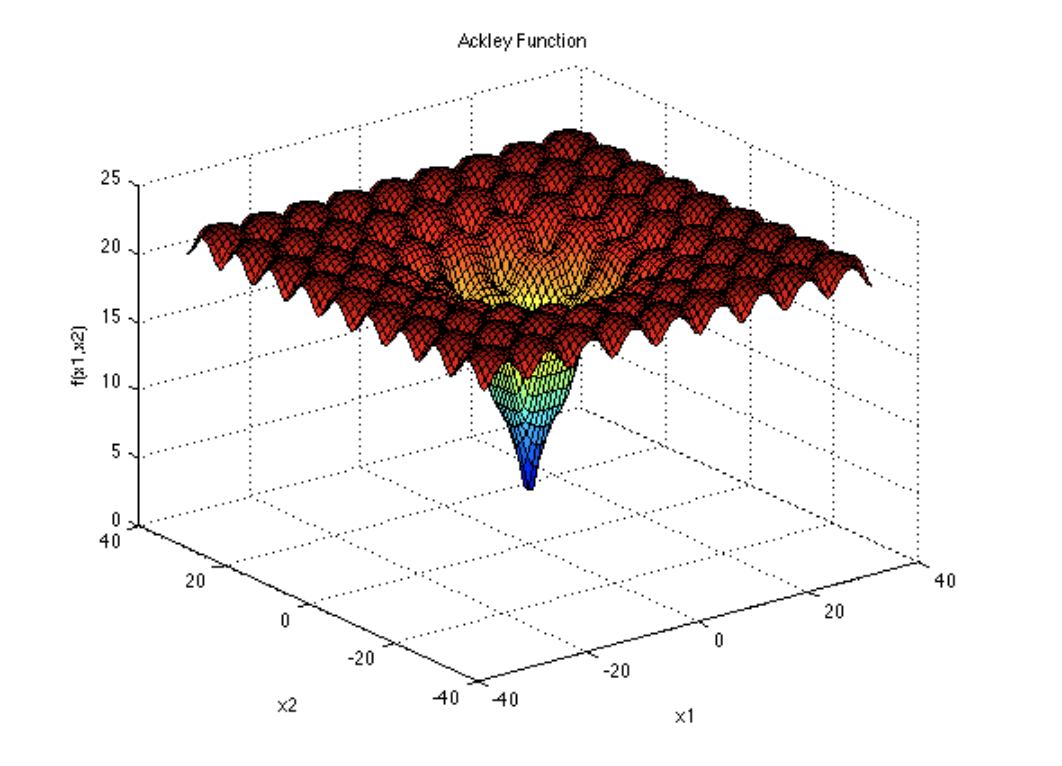
\includegraphics[width=0.65\linewidth]{figures/ackley.png} 
    \caption{Two variable Ackley function \cite{sfu_ackley_nodate}.}
    \label{fig:ackley}
\end{figure}
 
I added an integration test to \gls{ROLLO} that checks that a default \gls{ROLLO} 
simulation will find the Ackley function's global optimum point. 
If \gls{ROLLO} performed sub-optimally, it would return one of the Ackley 
function's many local minimums. 
\gls{ROLLO} successfully finds the global optimum point, and thus passes the 
integration test. 

\subsection{Binh and Korn Function}
The Binh and Korn function \cite{binh_mobes_1997} is a two-objective function:
\begin{align}
    Minimize &= \begin{cases}
        f_1 (x_1,x_2) &= 4x_1^2+4x_2^2 \\
        f_2 (x_1,x_2) &= (x_1-5)^2 + (x_2-5)^2 
    \end{cases} \\
    Such that &= \begin{cases}
        (x_1-8)^2 + (x_2+3)^2 \geq 7.7 \nonumber \\
        0 \leq x_1 \leq 5, 0 \leq x_2 \leq 3 \nonumber
    \end{cases}
\end{align}
We use it as a performance test for two-objective optimization.
Figure \ref{fig:binh_paretofront} shows the Binh and Korn function's pareto front.
\begin{figure}[]
    \centering
    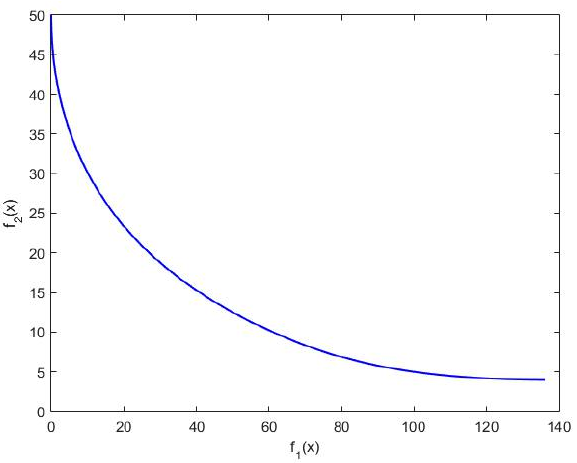
\includegraphics[width=0.7\linewidth]{binh-paretofront.png} 
    \caption{Pareto front of the Binh and Korn test function, taken from 
    \cite{bassi_statistics_2018}. }
    \label{fig:binh_paretofront}
\end{figure}
I use the hypervolume indicator to quantify the pareto front's goodness. 
The hypervolume indicator is one of the most used set-quality indicators for the 
assessment of stochastic multiobjective optimizers \cite{guerreiro_hypervolume_2020}.
The hypervolume indicator measures the volume (in the objective space) covered by 
non-dominated solutions for problems in which all objectives are to be 
minimized \cite{deb_multi-objective_2001}. 
For a two-dimensional problem, Figure \ref{fig:pareto_hypervolume} illustrates the 
hypervolume enclosed by the non-dominated solutions (A, B, C, D, E) and reference 
point, W, in the hatched region. 
\begin{figure}[]
    \centering
    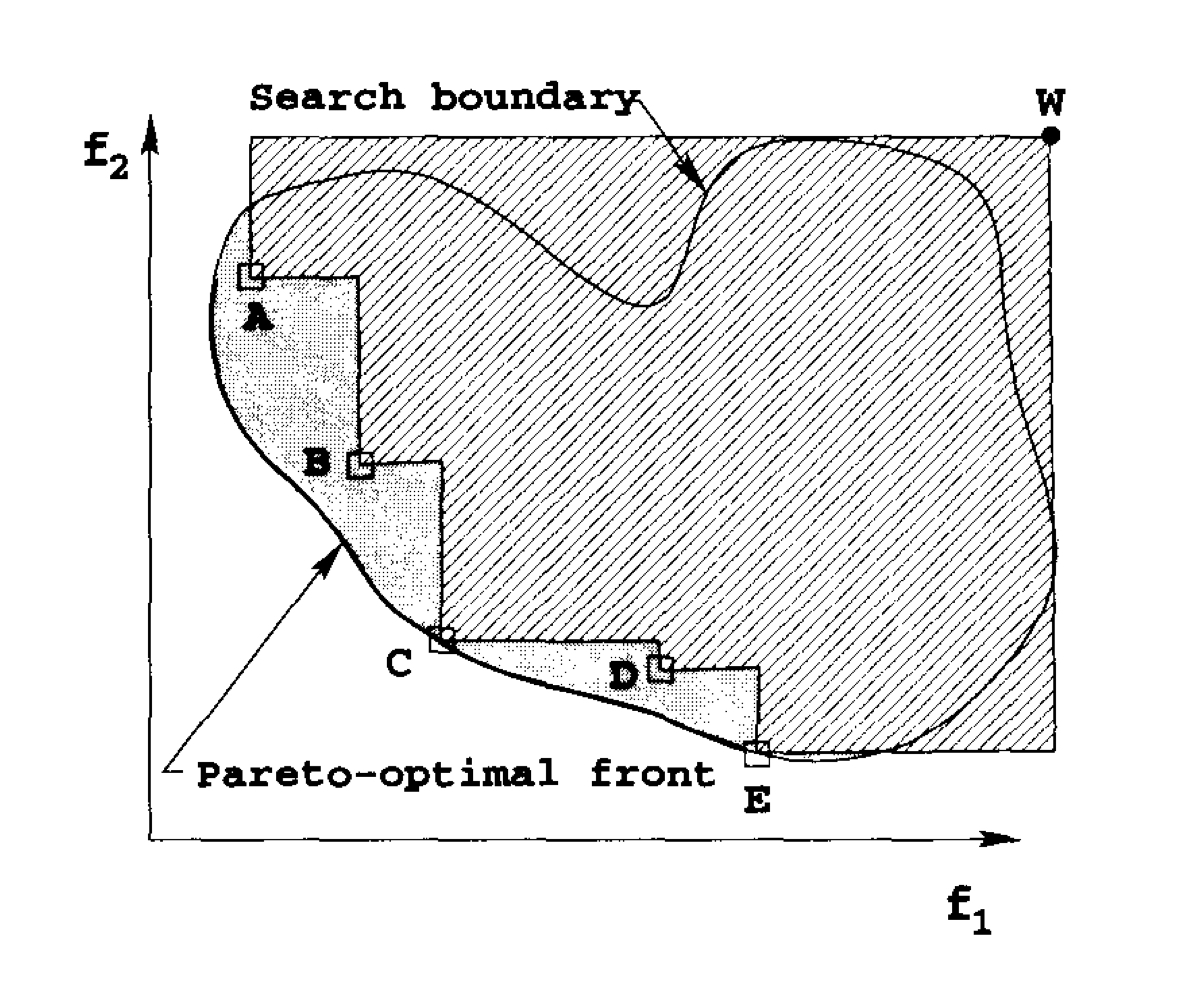
\includegraphics[width=0.7\linewidth]{pareto-hypervolume.png} 
    \caption{Example hypervolume enclosed by non-dominated solutions, taken from 
    \cite{deb_multi-objective_2001}.}
    \label{fig:pareto_hypervolume}
\end{figure}
I added an integration test to ROLLO that checks that a ROLLO simulation will 
find a hypervolume comparable to the ideal pareto front when minimizing the
Binh and Korn function. 

\subsection{Pu-239 Critical Bare Sphere}
To ensure \gls{ROLLO} works correctly while coupled with OpenMC, I run \gls{ROLLO} 
to find the critical radius for a $^{239}Pu$ bare sphere. 
The solution to this problem is well studied and available \cite{blanchard_updated_1999}. 
Blanchard et al reported that with MCNP4b code and ENDF/B-VI data library, the 
critical mass of a Pu239 bare sphere is 10.00 kg which corresponds to a diameter 
of 9.9cm \cite{blanchard_updated_1999}.
Figure \ref{fig:verification-sphere} shows the ROLLO input file for this verification 
problem. 
In the input file, I vary the radius between 1.0 and 8.0cm, with the objective of 
minimizing radius, while constraining the problem to have $k_{eff} >= 1.0$.
\begin{figure}[H]
    \begin{minted}[
        frame=lines,
        framesep=2mm,
        baselinestretch=1.2,
        fontsize=\footnotesize,
        linenos
        ]{json}
        {"control_variables": {
                "radius": {"min": 1.0, "max": 8.0}},
            "evaluators": {
                "openmc": {
                    "input_script": "critical_sphere.py",
                    "inputs": ["radius"],
                    "outputs": ["keff", "radius"],
                    "keep_files": false}},
            "constraints": {"keff": {"operator": [">="], "constrained_val": [1.0]}},
            "algorithm": {
                "parallel": "multiprocessing",
                "objective": ["min"],
                "optimized_variable": ["radius"]
            }}
    \end{minted}
    \caption{\acrfull{ROLLO} JSON input file for finding the minimum radius for 
    a $^{239}Pu$ Critical Bare Sphere.}
    \label{fig:verification-sphere}
\end{figure}
\pagebreak
Figure \ref{fig:critical_sphere.py} shows the OpenMC template used in the 
\gls{ROLLO} simulation. 
\begin{figure}[H]
    \begin{minted}[
        frame=lines,
        framesep=2mm,
        baselinestretch=1.2,
        fontsize=\footnotesize,
        linenos
        ]{python}
            import openmc 
            import numpy as np

            pu = openmc.Material()
            pu.set_density("g/cm3", 19.84)
            pu.add_nuclide("Pu239", 1)
            mats = openmc.Materials([pu])
            
            radius = {{radius}}
            
            fuel_sphere = openmc.Sphere(r=radius, boundary_type='vacuum')
            fuel_cell = openmc.Cell(fill=pu, region=-fuel_sphere)
            univ = openmc.Universe(cells=[fuel_cell])
            geom = openmc.Geometry(univ)
            
            settings = openmc.Settings()
            settings.batches = 100
            settings.inactive = 20
            settings.particles = 20000
            settings.temperature = {"multipole": True, "method": "interpolation"}
            
            mats.export_to_xml()
            geom.export_to_xml()
            settings.export_to_xml()
            openmc.run()
    \end{minted}
    \caption{OpenMC template input file used in ROLLO simulation to find the 
    minimum radius for a $^{239}Pu$ Critical Bare Sphere.}
    \label{fig:critical_sphere.py}
\end{figure}  

\gls{ROLLO} successfully finds the critical radius of the $^{239}Pu$ bare sphere 
to be 4.9856cm which corresponds to approximately a 9.9cm diameter. 
The critical sphere's $k_{eff}$ value is 1.00919 $\pm$ 0.00048. 
Figure \ref{fig:verification-radius} and \ref{fig:verification-keff} show the 
radius and $k_{eff}$ evolution through the evolutionary algorithm's 
generations. 
They demonstrate how the average radius and $k_{eff}$ converge
towards the critical radius while keeping $k_{eff} > 1$ with improvements from 
each generation.
\begin{figure}[]
    \centering
    \begin{subfigure}{\textwidth}
    \makebox[\textwidth][c]{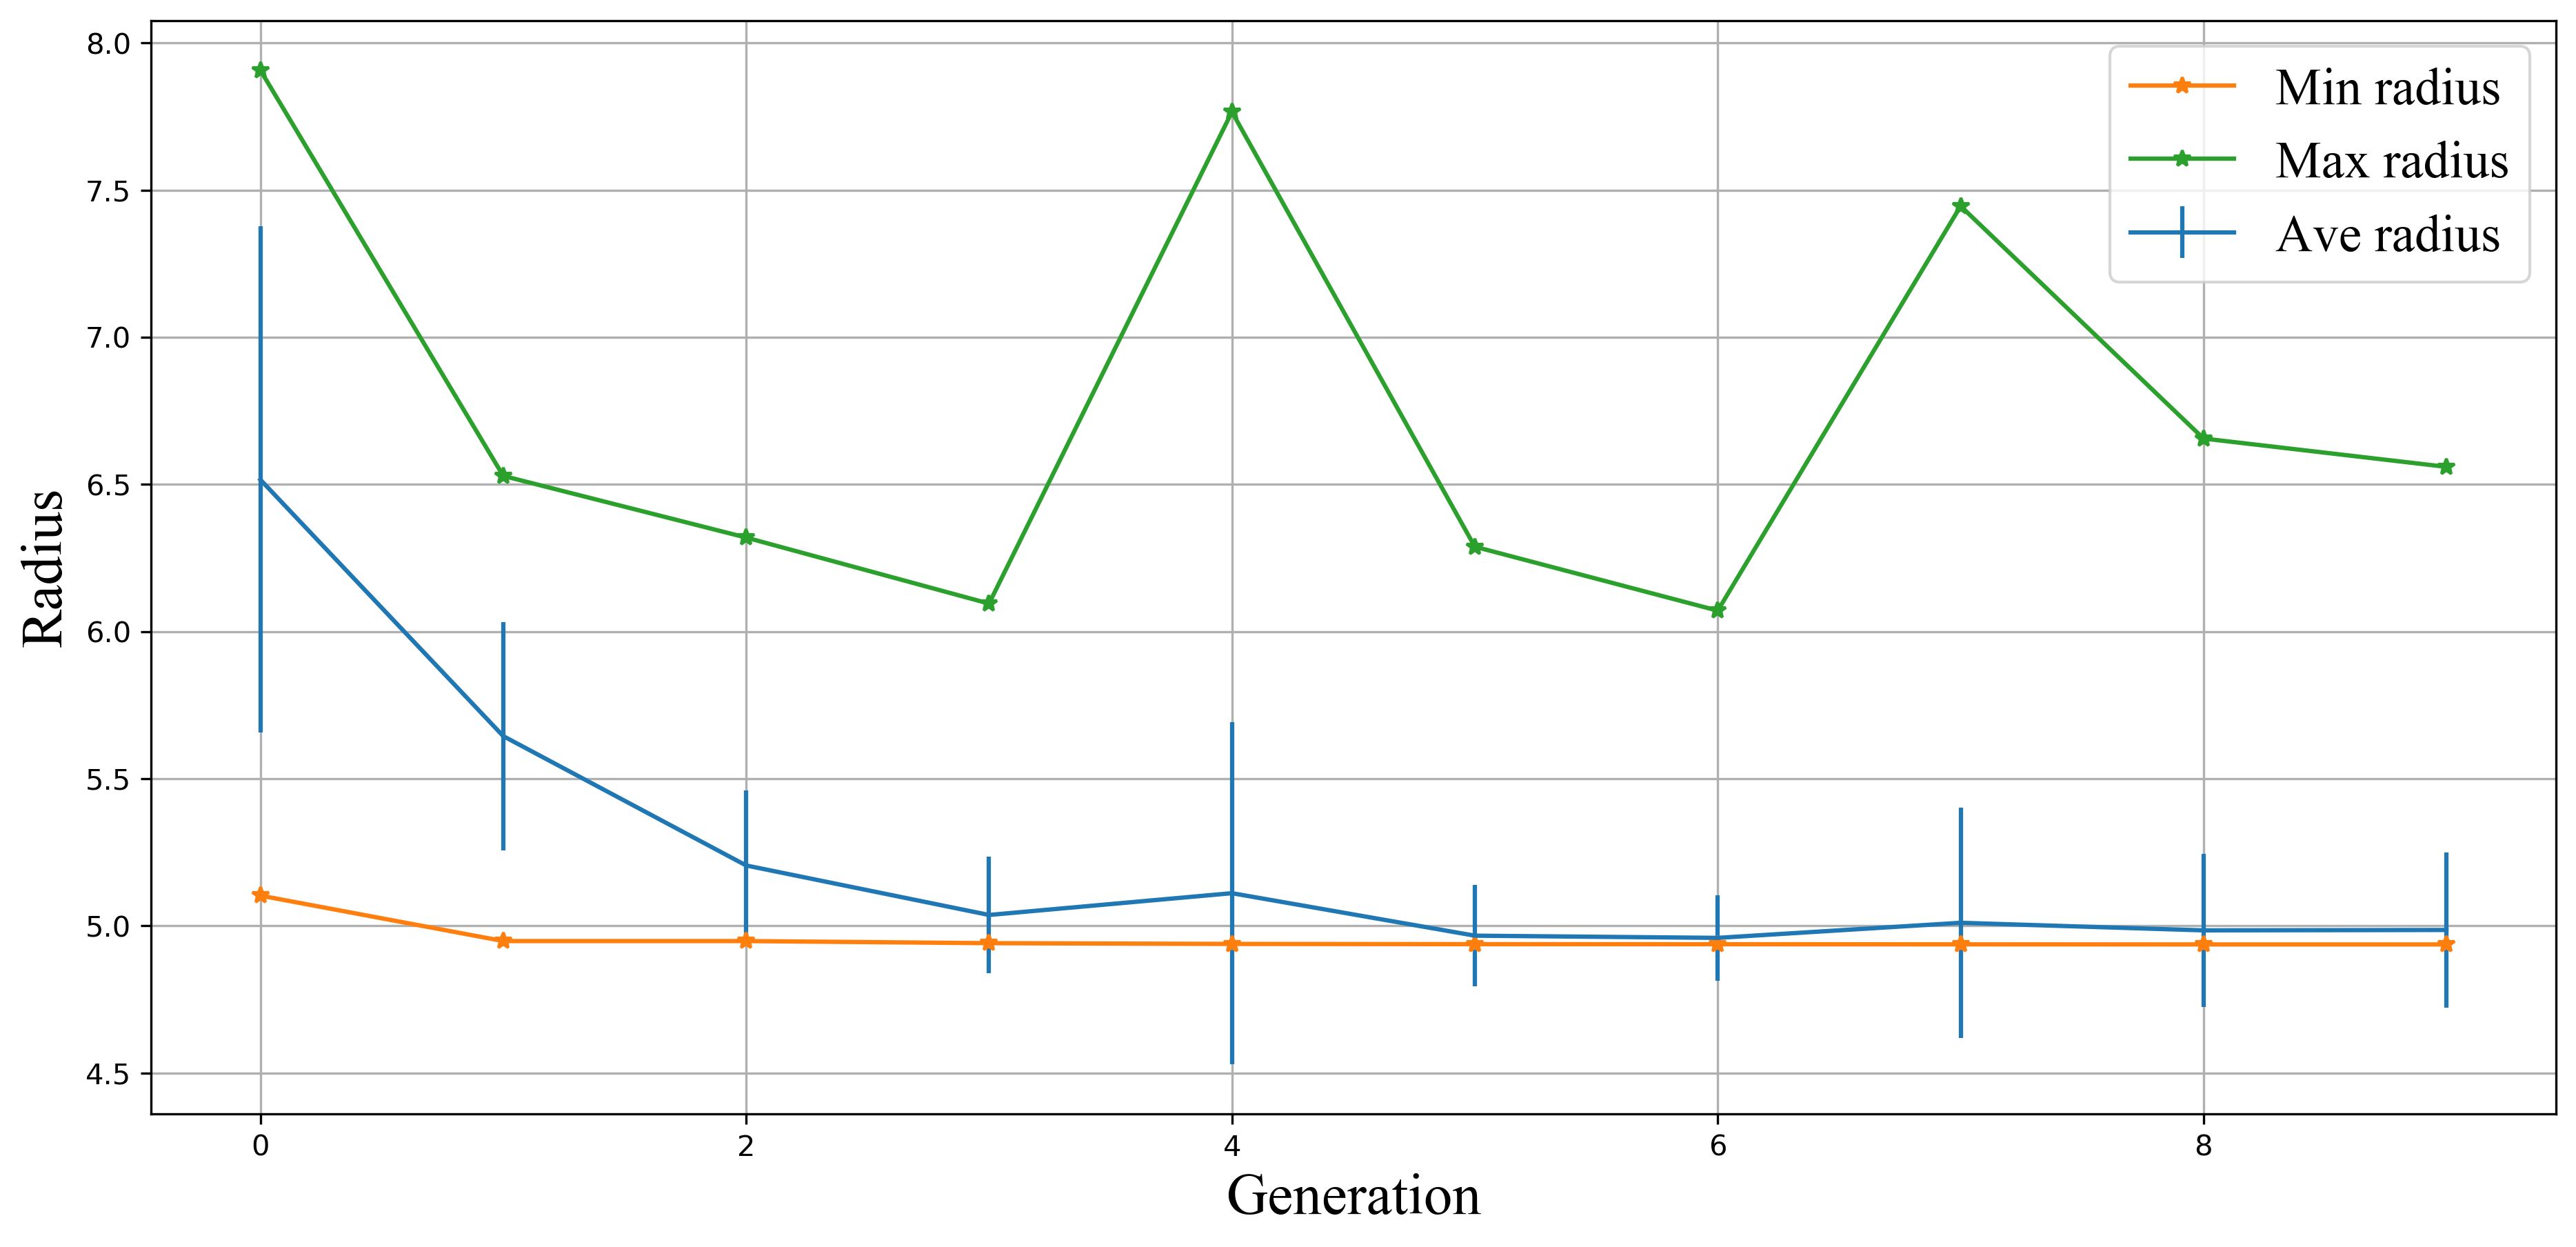
\includegraphics[width=1.1\linewidth]{verification-radius.png}} 
    \caption{Minimum, average, and maximum radius values evolution.}
    \label{fig:verification-radius}
    \end{subfigure}
    \begin{subfigure}{\textwidth}
        \makebox[\textwidth][c]{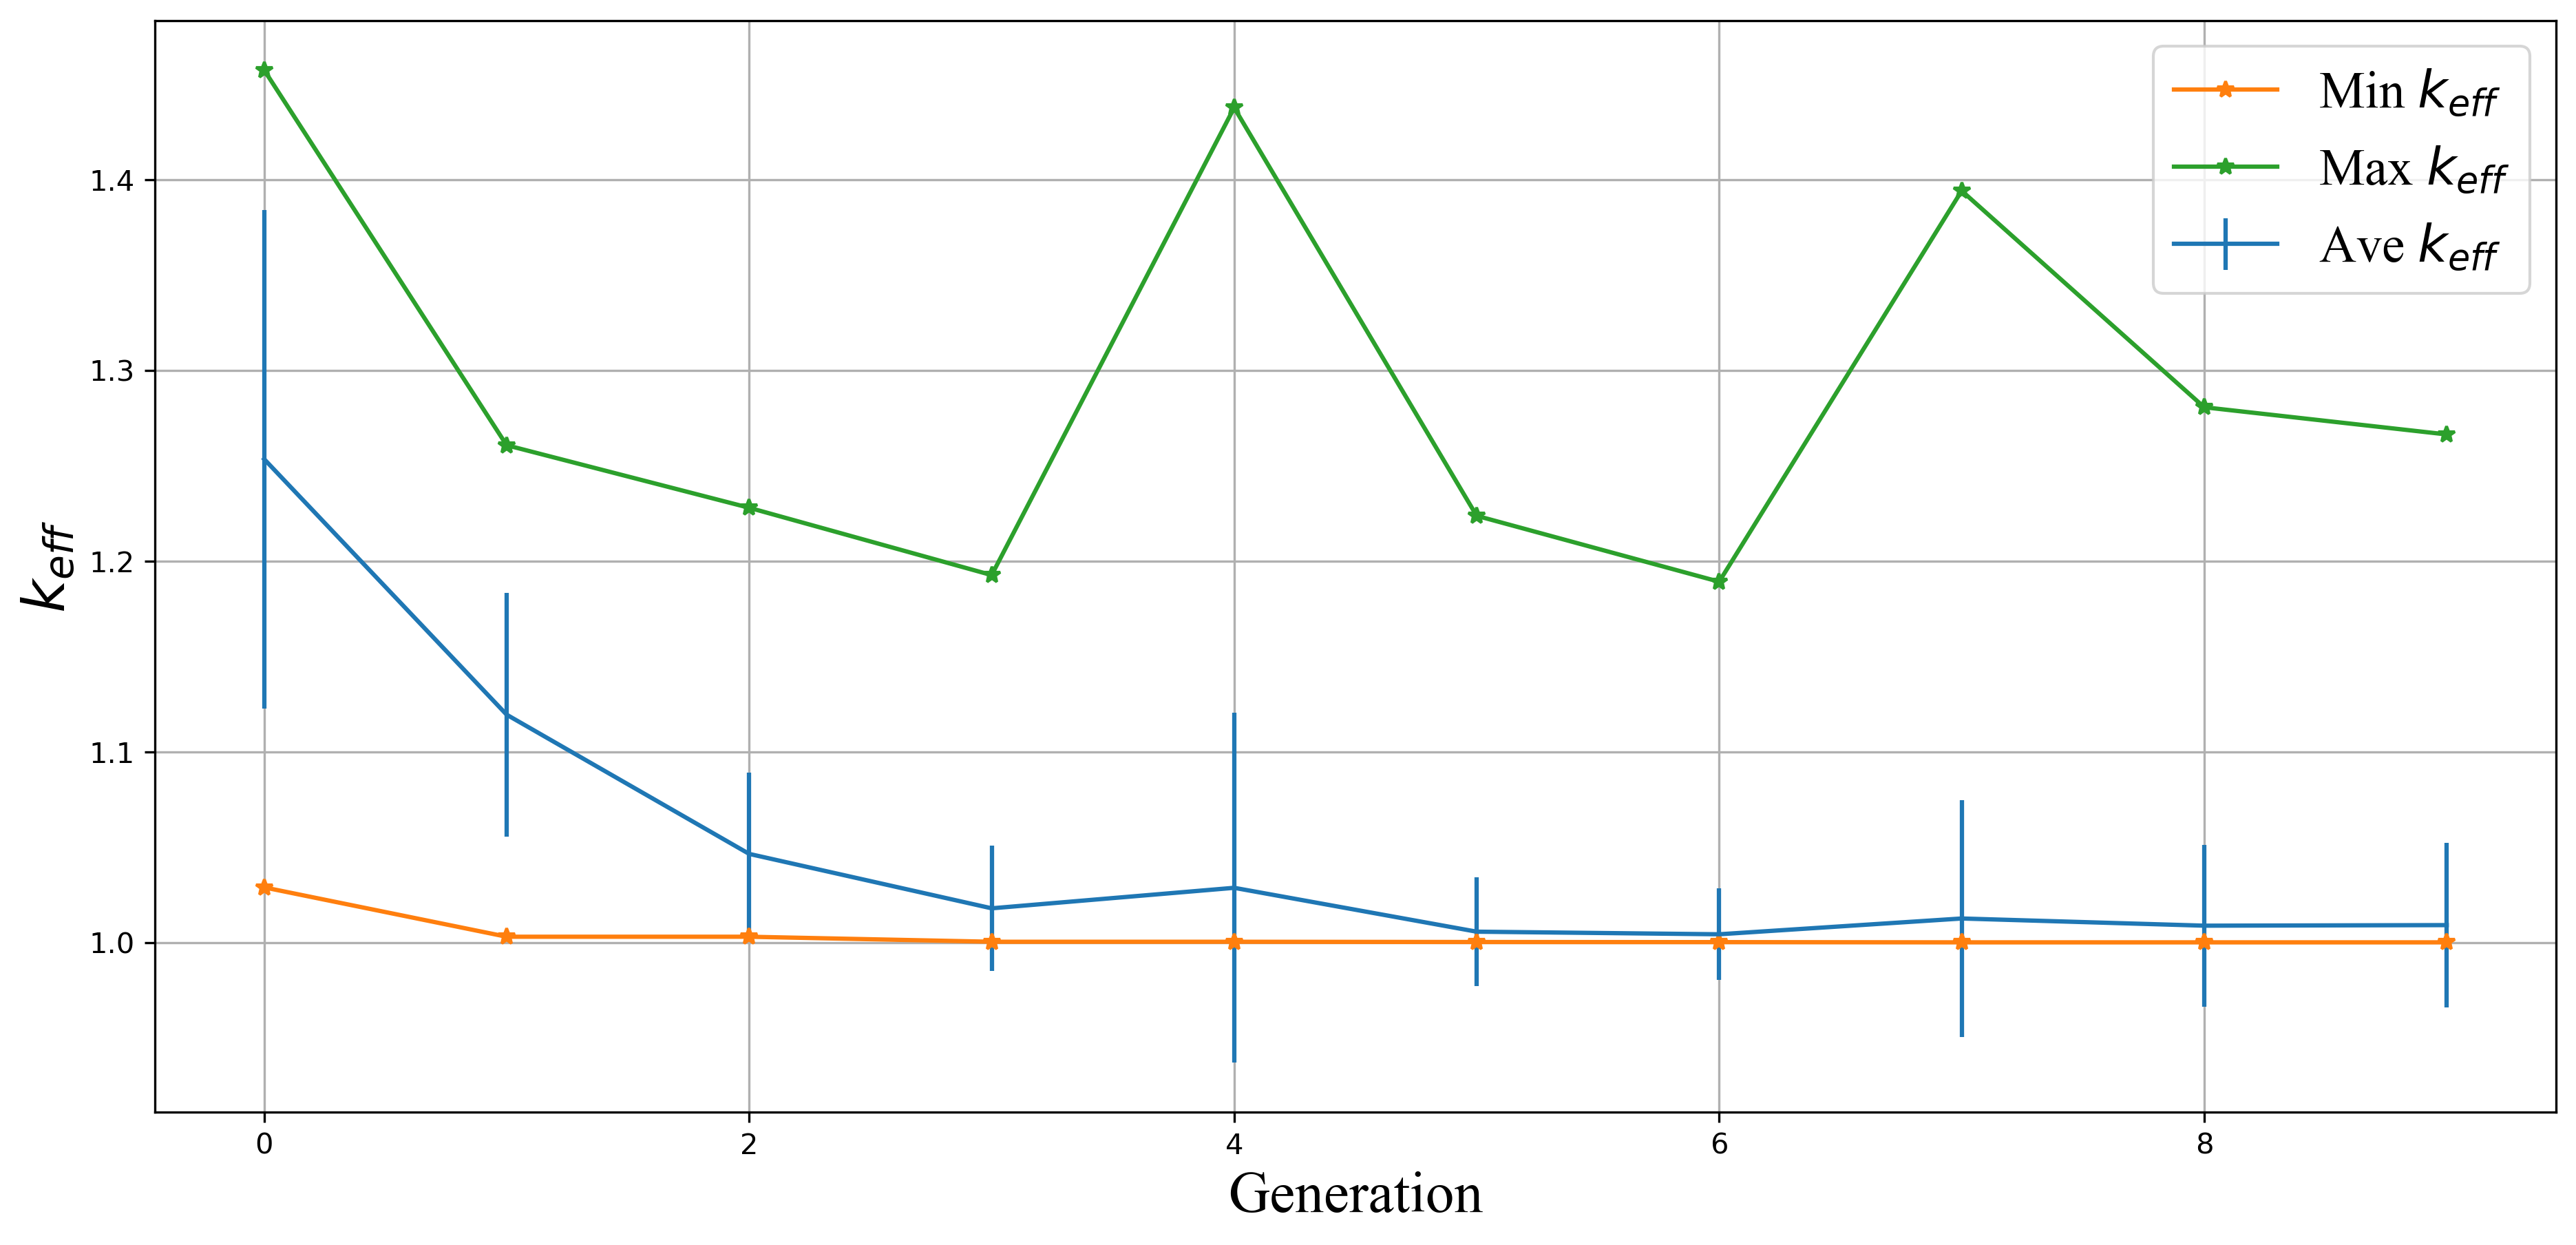
\includegraphics[width=1.1\linewidth]{verification-keff.png}}
        \caption{Minimum, average, and maximum $k_{eff}$ values evolution.}
        \label{fig:verification-keff}
    \end{subfigure}
    \caption{Results for each generation for \gls{ROLLO}'s genetic algorithm optimization 
    to the find the critical radius of a  $^{239}Pu$ bare sphere.}
\end{figure}

\section{ROLLO Stopping Criteria}
ROLLO's evolutionary algorithm stopping criterion is defined by the
\texttt{generations} input parameter.  
Each nuclear reactor model's evaluation is computationally intensive. 
Users will most likely be constrained by total available compute time. 
Therefore, rather than setting a results-based stopping criterion, ROLLO enables 
users to define the \texttt{generations} and \texttt{pop$\_$size} based on the 
amount of compute time available to them: 
\begin{align}
    t_{total} &= t_{eval} \times gen \times pop 
\intertext{where}
    t_{total} &= \mbox{Total compute time available} \nonumber \\
    t_{eval} &= \mbox{compute time per nuclear reactor model evaluation} \nonumber \\
    gen &= \mbox{total number of generations in optimization process} \nonumber \\
    pop &= \mbox{population size in optimization process} \nonumber
\end{align} 

\subsection{Convergence}
% highlight that we're narrowing the search space. 
% it's up to the decision maker to determine if the problem is converged 
% enough. 
ROLLO does not utilize a mathematical expression to evaluate problem convergence. 
The complexity of reactor design optimization means that there is no single 
indicator that determines if convergence is met. 
Instead, ROLLO's purpose is to help the human reactor designer to narrow down 
the search space. 
When a ROLLO run is completed, the user plots the objectives convergence and 
pareto front (for multi-objective simulations) to evaluate if they are confident 
about the final solution set. 
If not, the user can easily restart the optimization simulation using the 
\texttt{checkpoint.pkl} file and run the problem for a few more generations. 

\section{Summary}
This chapter described the \acrfull{ROLLO} framework developed as
preliminary work for the proposed PhD scope.
\gls{ROLLO} is a Python package that applies evolutionary algorithm 
optimization techniques to nuclear reactor design using the \acrfull{DEAP} 
module, OpenMC, and Moltres. 
The motivation for \gls{ROLLO} is to enable reactor designers to utilize 
robust evolutionary algorithm optimization methods without going 
through the cumbersome process of setting up a genetic algorithm framework,
selecting appropriate hyperparameters, and setting up its parallelization. 
\gls{ROLLO} is designed to be effective, flexible, open-source, parallel, 
reproducible, and usable. 
\gls{ROLLO} is hosted on Github \cite{chee_rollo_2021}. 